\section{Прочие аспекты}\label{sec:ch2/sec4}

Использование регенерированного урана, помимо возможностей расширения ресурсной базы и сокращения отходов, необходимо рассмотреть и с иных позиций. Так, переработка ОЯТ для последующего использования зачастую рассматривается как нежелательная опция с позиций нераспространения ядерного оружия (позиция США в рамках GNEP), а технология газовой центрифуги и материал класса НОУ на сегодня рассматриваются экспертами как наиболее чувствительные \cite{nevinicaPovyshenieZashchishchennostiEksportnyh}. То есть, расширение применения двух ключевых технологии для возврата урана в цикл - гидрометаллургического восстановления и газоцентрифужного каскадного обогащения представляется, на первый взгляд, негативным с точки зрения вопроса сдерживания распространения ядерного оружия. Однако, если производство ядерного топлива ограничивается странами - глобальными лидерами в ЯЭ (как, к примеру, в рамках российской инициативы по созданию системы международных центров по предоставлению услуг ядерного топливного цикла), а неядерным державам, поставляется топливо на основе регенерата урана, ситуация в корне меняется. Благодаря нейтроно-физическим свойствам такого топлива, вариант его переключения представляется гораздо менее осуществимым. Это обусловлено как неизбежным высоким радиационным воздействием в случае операции переключения ядерного материала, сопровождающейся необходимостью его конверсии (несколько стадий) и обогащения, так и легкостью детектирования изъятия даже малых количеств делящегося материала. Помимо резкого снижения привлекательности материала на основе регенерата для создания ядерного уранового заряда, присутствие в нем U-236 значительным образом повышает выходную концентрацию Pu-238 в изотопном векторе плутония, уменьшая возможность его немирного переключения. Так, в работе \cite{solovevAnalizYadernogoToplivnogo2019} показано, что рециклирование РЕМИКС-топлива, приводит к накоплению четных изотопов в плутониевой фракции, повышая защищенность от несанкционированного переключения.


\subsection{Ядерное нераспространение. Анализ сценариев переключения}\label{sec:ch2/sec4.1}

Рассмотрен модельный сценарий переключения ядерного материала из топлива легководного реактора типа ВВЭР-1000 или ВВЭР-1200,  изготовленного из регенерированного урана. Предполагали, что АЭС находится под гарантиями МАГАТЭ. Технической целью гарантий является предотвращение или своевременное обнаружение переключения значимого количества ядерных материалов (требования своевременности обнаружения переключения значимого количества ЯМ зависят от  его категории) \cite{ermakovVozmozhnyeProceduryGarantiy1987}. Так, в соответствие с \cite{ermakovVozmozhnyeProceduryGarantiy1987}, технической целью гарантий МАГАТЭ применительно к реактору ВВЭР-1000 является обнаружение переключения в течение года такого количества низкообогащенного урана, которое содержит более 75 кг $^{235}$U.
...с помощью:  надкритических центрифуг TC-12 компании URENCO \cite{borisevichIdealOptimumCascades2014}. 


Представленные зависимости наглядно демонстрируют, что период между инспекциями является временем, вполне достаточным для переключения. За рамками работы мы оставили вопрос химической конверсии (превращения оксидов U в фториды U и наоборот (и в металл)) \cite{orlovDesublimationPurificationTransporting2017}, однако это одна из необходимых технологий, требуемых для обогащения урана. 


\section{Оптимизация каскадов для полного возврата регенерата}\label{sec:ch2/sec5}
\subsection{Выбор оптимизационных критериев}\label{sec:ch2/sec5.1}

\paragraph{Оценка себестоимости}
Методика оценки в текущих ценах с портала UxC.
\paragraph{Синтетический энергетический показатель}
Сравнение эффективности схем по энергетическому показателю \cite{2019}.
\paragraph{Максимизация вовлечения делящегося изотопа}
Степень извлечения $^{235}$U как ключевой показатель эффективности.
\paragraph{Минимизация соотношения U-232 к U-235 в продукте}

\subsection{Процедура оптимизации каскадов для полного возврата регенерата}\label{sec:ch2/sec5.2}
Выбор схемы для осуществления полного возврата связан с оптимизацией вышеозначенным критериям. Для возможности работы над единой схемой, объединяющей различные варианты обращения с потоком, образующимся на легком конце каскада с индексом 2, предложена схема \ref{fig:Total scheme}. Так как она включает в себя ранее разработанные конфигурации, представленные на рисунках \ref{fig:Tomsk} и \ref{fig:patent}, целесообразно проводить оптимизацию с ее помощью. Полученный результат в этом случае будет сопутствовать оптимальный режим обращения с производимой грязной смесью потока, получаемого на выходе из второго каскда (через \ref{fig:Tomsk} или же через \ref{fig:patent}).
Добавим, что процедура оптимизации может быть выполнена в постановке многокритериальной задачи, а расчетный код может быть оформлен в качестве программного комплекса, выступающего системой поддержки принятия решений.

\begin{figure}[ht]
  \centerfloat{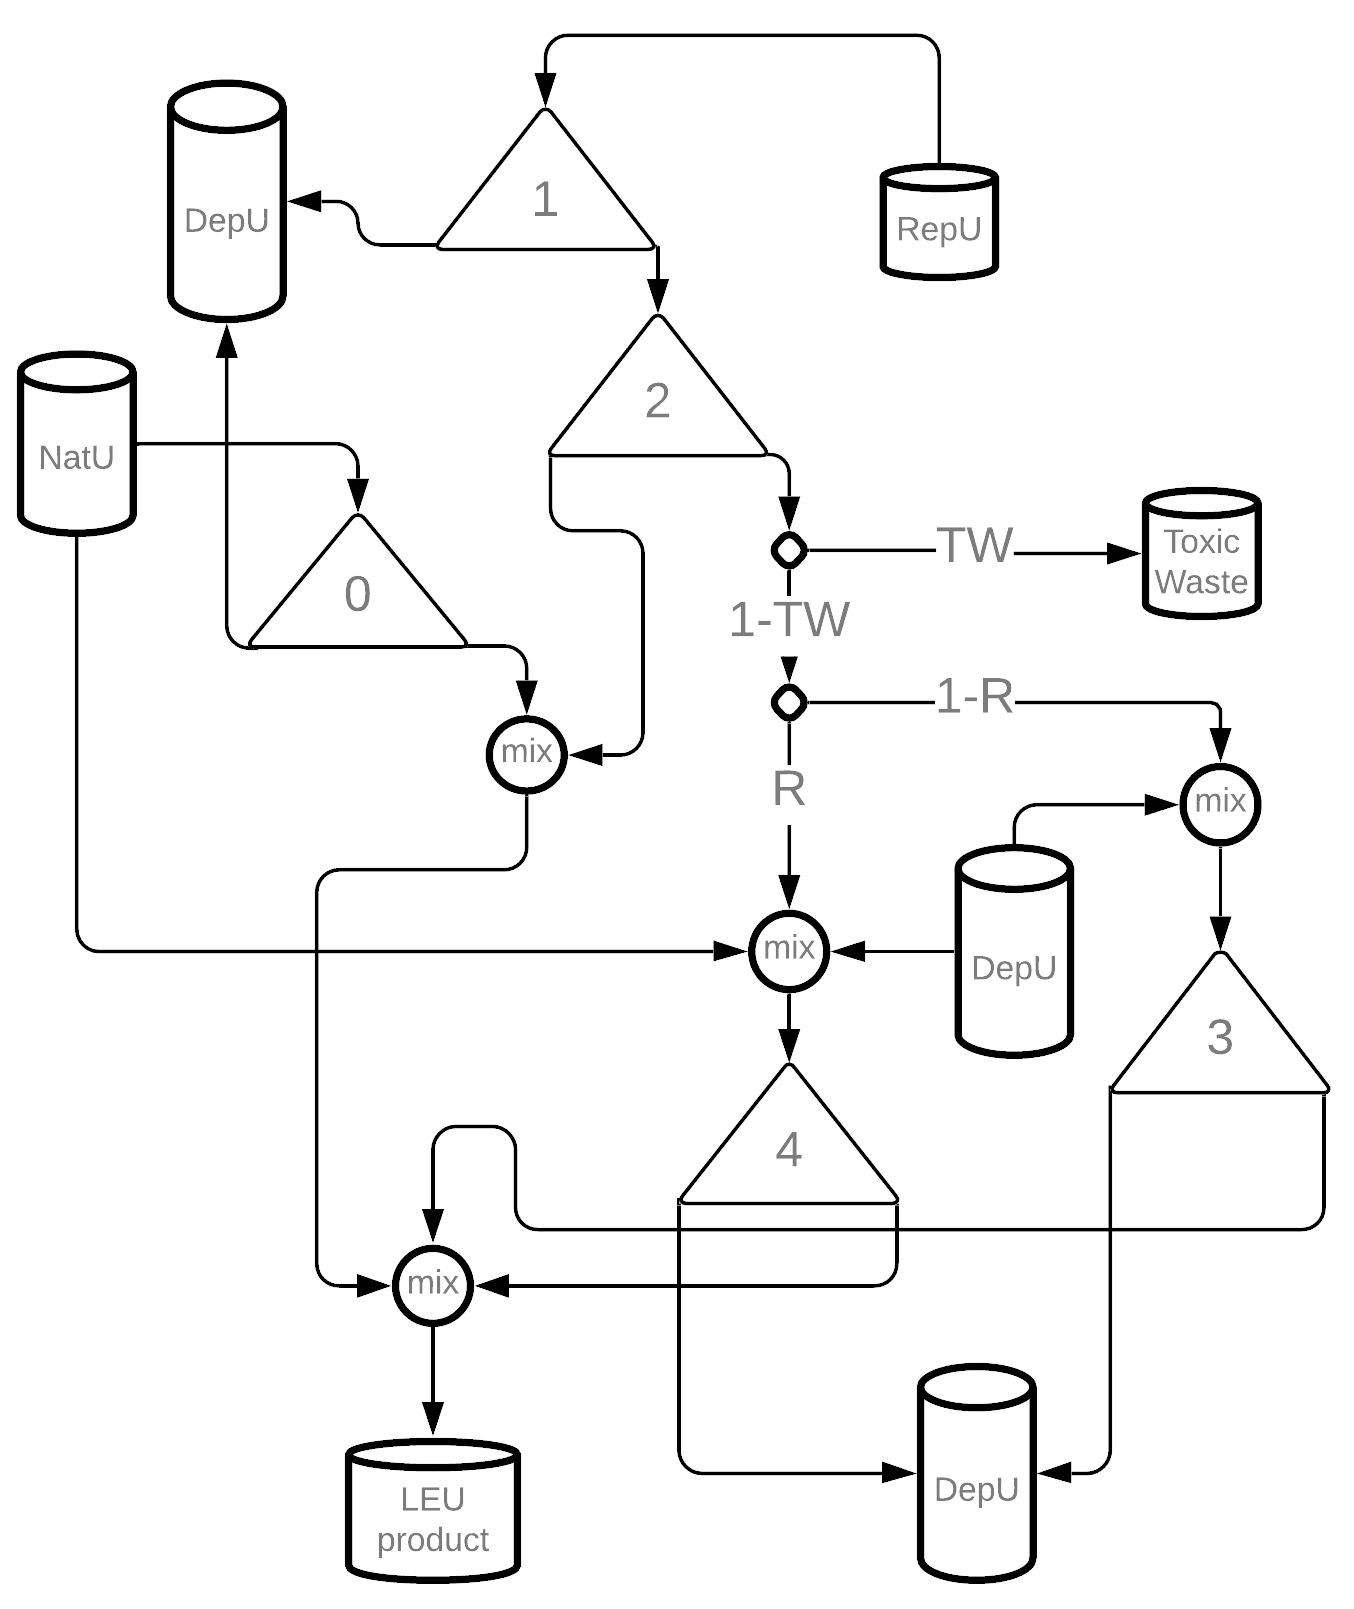
\includegraphics[scale=0.3]{cascades/Total scheme}}
  \caption{Пятикаскадная схема}\label{fig:Total scheme}
\end{figure}

Отметим, что для сравнения схемы с бенчмарком -- ординарным каскадом, необходимо усреднить отвальные концентрации, получаемые в тяжелых фракциях входящих в составную конфигурацию каскадов, и использовать полученное значение концентрации $^{235}$U в отвале ординарного каскада на природном уране, проводя вычисление потребляемых Единиц Работы Разделения (ЕРР).




\subsubsection{Поступенный расчет}
Стоит упомянуть, что существует альтернативный подход к каскадному расчету, когда набор из шести уравнений включает 10 основных внутренних параметров:

$L_{i}, C_{i}, L_{i}^{\prime}, C_{i}^{\prime}, L_{i}^{\prime \prime}, C_{i}^{\prime \prime}, q_{i}, \theta_{i}, N_{i}, l_{i}$,

где $L_{i}, L_{i}^{\prime}, L_{i}^{\prime \prime}$ и $C_{i}, C_{i}^{\prime}, C_{i}^{\prime \prime}$ -- 
это потоки питания, продукта и отвала и их концентрации соответственно; $q_{i}$ -- коэффициент разделения; $\theta$ -- коэффициент деления потока на ступени (срез); $N_{i}$ -- число ступеней; и $l_{i}$ -- поток питания отдельной центрифуги.

Эти параметры связаны шестью уравнениями:
$\begin{array}{c}
  {L_{i}^{\prime}+L_{i}^{\prime \prime}=L_{i}} \\
  {L_{i}^{\prime} C_{i}^{\prime}+L_{i}^{\prime \prime} C_{i}^{\prime \prime}=L_{i} C_{i}} \\
  {q_{i}=\frac{(1-C_{i}^{\prime \prime}) C_{i}^{\prime}}{(1-C_{i}^{\prime}) C_{i}^{\prime \prime}}} \\
  {q_{i}=q_{i}\left(l_{i}, \theta_{i}\right)} \\
  {\theta_{i}=\frac{L_{i}^{\prime}}{L_{i}}} \\
  {l_{i}=\frac{L_{i}}{N_{i}}}
\end{array}$

Помимо этих 6$n$ соотношений, описывающих отдельные ступени, необходимо учитывать уравнение, связывающее межкаскадные потоки -- балансные уравнения, вид которых зависит от рассматриваемой схемы коммутации ступеней. Для каскада, показанного на рис. 1, эти уравнения записаны в виде:

$\begin{array}{c}
  {L_{1}=L_{2}^{\prime \prime}, \ldots ; L_{i}=L_{i-2}^{\prime}+L_{i+1}^{\prime \prime}, \ldots ;} \\
  {L_{1} C_{1}=L_{2}^{\prime \prime} C_{2}^{\prime \prime}, \ldots ; L_{i} C_{i}=L_{i-2}^{\prime} C_{i-2}^{\prime}+L_{i+1}^{\prime \prime} C_{i+1}^{\prime \prime}, \ldots}
\end{array}$

В дополнение к этим соотношениям необходимо учитывать граничные условия, относящиеся к внешним и внутренним параметрам. Например для симметричного противоточного каскада, они выражаются соотношениями: 
$P=L_{n}^{\prime} ; C_{P}=C_{n}^{\prime} ; W=L_{1}^{\prime \prime} ; C_{W}=C_{1}^{\prime \prime}$

, которые выполняются для каждой ступени каскада \cite{palkinDeterminationOptimalParameters2012}. Эти уравнения описывают отношения между соседними ступенями и, опираясь на ряд граничных условий, могут служить эффективной репрезентацией каскада. 






\textcolor{red}{В презентации Щелканова с семинара ТВЭЛ, ASTM C996 ограничивает присутствие $^{232}$U на уровне $5\cdot10^{-6}$\%, а в презентации от TENEX -- 5 ppb, то есть $5\cdot10^{-7}$\%.}









